\documentclass[10pt,twocolumn]{article}



\usepackage[utf8]{inputenc}
\usepackage{amsmath}
%\usepackage{ae}
\usepackage{graphicx}
\usepackage{color}
%\usepackage{bbm}
%\usepackage[swedish]{babel}
\newcommand{\N}{\ensuremath{\mathbbm{N}}}
\newcommand{\Z}{\ensuremath{\mathbbm{Z}}}
\newcommand{\Q}{\ensuremath{\mathbbm{Q}}}
\newcommand{\R}{\ensuremath{\mathbbm{R}}}
\newcommand{\C}{\ensuremath{\mathbbm{C}}}
\newcommand{\rd}{\ensuremath{\mathrm{d}}}
\newcommand{\id}{\ensuremath{\,\rd}}
\newcommand{\ket}[1]{|#1\rangle}
\newcommand{\bra}[1]{\langle#1|}
\newcommand{\braket}[2]{\bra{#1}#2\rangle}
\newcommand{\bracket}[3]{\bra{#1}#2\ket{#3}}

\title{Speed and Lifetime Measurement of Cosmic Muons}
\author{Jonathan Lindgren \and Petter Säterskog}
\newpage
\usepackage[margin=0.5in]{geometry}
\begin{document}

\maketitle
\section{Introduction}

\section{Experimental setup}
In this experiment we used three plastic scintillator detectors located on top of each other. The upper two detectors, \emph{P1} and \emph{P2}, are flat. They are separated by a gap of 2.4 meters with P1 on the top. The lowest detector, \emph{B}, was bigger to be able to fully stop the muons. When a muon goes through one of the detectors we will get a light pulse that is amplified by a photo multiplier tube (PMT). The time difference between pulses from P1 and P2 can be used for determining the speed of the muons. These PMT signals were reshaped by a constant fraction discriminator (CFD) and then sent to a time to amplitude converter (TAC). The signal from P1 was used to start the TAC and the signal from P2 to stop it. See Figure \ref{setup}. A computer recorded the output of the TAC. The relationship of the channel recorded by the computer and the time delay measured by the TAC was determined by sending pulses of known delays to its start and stop inputs.\\  %ev bild av tCal
The difference of the delays of the signals from P1 and P2 to the start and stop of the TAC, $\Delta t$, is not known due to the possible differences in the PMTs and cabelings. A radioactive $^{60}$Co sample was placed below P2 for calibration. It releases two photons simultaneously so that they can be detected in both P1 and P2. The pulses from P2 were delayed enough for both the muons going through P1 and then P2 and the photons going the opposite direction to be timed by the TAC. Plotting the measured times as a histogram shows two peaks. The first peak is from the photons and the later from the muons. The shape and position of the photon peak in the spectrum 


To determine the lifetime of the muons we used on scintillator and the barrel detector. Coincidence between the barrel and the scintillator were used to be able to identify signals from muons that went through the scintillator and then absorbed in the barrel. The barrel will first give a signal from the energy absorbed when slowing down the muon and another signal when it decays. The start and stop signals are separated by an AND respectively AND-NOT gate with the scintillator signal, see fig().



\section{Results}
To determine the lifetime of the muon we fitted an exponential distribution to the measured data. However, the Time To Amplitude converter could not measure very well for small and large lifetimes, thus we only considered a limited interval $[t_1,t_2]$ and this has to be taken into account into the propability distribution. By looking at the spectrum it is reasonable to also add a constant noise $C$, so the distribution is
\begin{equation}
f(t)=\frac{\exp{(-t/\tau)}+C}{\tau\exp{(-t_1/\tau)}-\tau\exp{(-t_2/\tau)}+C(t_2-t_1)}\label{pdf}
\end{equation}

To determine $\tau$ and $C$ for our measured data the likelyhood function $L=\prod_i f(t_i)$ was maximized yielding $\tau=2.07$ $\mu$s. \newline

The statistical error was determined by sampling many different simulated sets of data points by using the distribution \eqref{pdf} and then calculate the standard deviation of these sets. The result was a standard deviation $\sigma=0.02$ $\mu$s. \newline

By applying the same method it is also possible to verify that the obtained constant noise is not just statistical fluctuations. Maximizing the likelyhood function with respect to the lifetime but with the constant noise set to zero a lifetime of $2.21$ $\mu$s is obtained. Using this lifetime to sample new sets of data points, and then fitting the distribution \eqref{pdf} to these data points it is possible to obtain the expected size of the statistical noise. This gives a simulated mean noise (the propability of a measure data point coming from noise) of $\approx1.6\cdot 10^{-3}$ with standard deviation $\approx1.8\cdot 10^{-3}$ which is unreasonably small compared to the noise of the data which is about $0.034$. It is thus clear that this can not be explained by statistical fluctuations and must be taken into account in the model as a constant background noise.

\subsection{Speed Measurement}

\begin{figure}
\centering
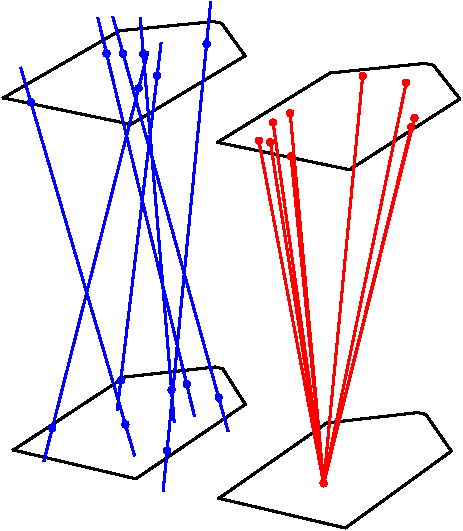
\includegraphics[width=6cm]{mc-crop.pdf}
\caption{Differential cross-section calculated by numerical integration.}
\label{cc}
\end{figure}

\section{Conclusions}
The obtained lifetime for the muon is slightly lower than the accepted value of $2.2$ $\mu$s which is not even in our error margin. However, this can be explained by the fact that there are two muons, $\mu^+$ and $\mu^-$, which doesnt have the same lifetimes in the detector material \cite{}. $\mu^+$ has the same lifetime as in vacuum, while $\mu^-$ has a lifetime of about $2.0$ $\mu$s. The size of the measurement data obtained in this experiment is too small to be able to separate these two exponential distributions.


% Figurer inkluderade som eps-filer
%% \begin{figure}\centering
%% 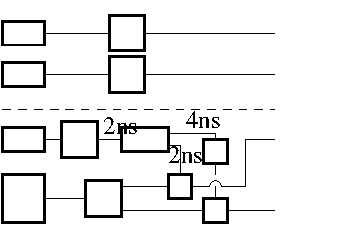
\includegraphics{speed.pdf}
%% \caption{\label{figuren} Perioden $T$ som funktion av pendellängden.}
%% \end{figure}

% Figurer inkluderade med xfigs postscript+latex

\begin{figure}[h]
\input{speed.pspdftex}
\caption{\label{setup} Schematic diagram of the different operations acting on the input signals.}
\end{figure}

\end{document}
